\documentclass{article}
\usepackage{graphicx} % Required for inserting images
\usepackage[T1]{fontenc}
\usepackage[polish]{babel}
\usepackage[utf8]{inputenc}
\usepackage[a4paper, total={6in, 8in}]{geometry}
\usepackage{hyperref}
\usepackage{csquotes}
\usepackage{flafter}
\usepackage{float}
\usepackage{pgfplots}
\usepackage{multirow}
\usepackage{colortbl}
\usepackage{xpatch}
\usepackage{xcolor}
\usepackage{realboxes}

\usepackage{listings}

%New colors defined below
\definecolor{mygray}{rgb}{0.8,0.8,0.8}
\lstset{
  basicstyle=\ttfamily,
  backgroundcolor=\color{mygray},
}
\makeatletter
\xpretocmd\lstinline{\Colorbox{mygray}\bgroup\appto\lst@DeInit{\egroup}}{}{}
\makeatother

\definecolor{codegreen}{rgb}{0,0.6,0}
\definecolor{codegray}{rgb}{0.5,0.5,0.5}
\definecolor{codepurple}{rgb}{0.58,0,0.82}
\definecolor{backcolour}{rgb}{0.95,0.95,0.92}

%Code listing style named "mystyle"
\lstdefinestyle{mystyle}{
  backgroundcolor=\color{backcolour},   commentstyle=\color{codegreen},
  keywordstyle=\color{magenta},
  numberstyle=\tiny\color{codegray},
  stringstyle=\color{codepurple},
  basicstyle=\ttfamily\footnotesize,
  breakatwhitespace=false,         
  breaklines=true,                 
  captionpos=b,                    
  keepspaces=true,                 
  numbers=left,                    
  numbersep=5pt,                  
  showspaces=false,                
  showstringspaces=false,
  showtabs=false,                  
  tabsize=2
}

%"mystyle" code listing set
\lstset{style=mystyle}

\title{Kultura DevOps i współczesne rozwiązania CI/CD}
\author{Aleksander Błaszkiewicz}
\date{Styczeń 2024}

\begin{document}

\maketitle
\newpage
\tableofcontents
\newpage

\section{Wstęp}
Kultura DevOps reprezentuje syntezę filozofii, praktyk oraz narzędzi, które są kluczowe w zwiększaniu zdolności organizacji do efektywnego dostarczania aplikacji i usług w akcelerowanym tempie. Ta koncepcja ewoluowała jako odpowiedź na rosnącą potrzebę lepszej komunikacji, współpracy i integracji między działami rozwoju oprogramowania (Dev) i operacjami IT (Ops).

Za rok, w którym narodziła się ta kultura uważa się rok 2009. To wtedy John Allspaw (starszy wiceprezes ds. operacji technicznych) oraz Paul Hammond (dyrektor inżynieryjny) wygłosili słynną prezentację "10+ Deploys per Day: Dev and Ops Cooperation at Flickr"\cite{flickr}. Z kolei za ojca tej kultury uważa się Patricka Deboisa - który zainspirowany prezentacją zorganizował własną konferencję o nazwie DevOpsDays, która popularna jest aż do dzisiaj \cite{devOpsDays}.

Rozwój tej kultury, chociaż silnie związany z programowaniem, wydaje się być opóźniony w stosunku do ewolucji samego programowania. Kultura DevOps, będąc reakcją na dynamiczny rozwój branży programistycznej, dopiero niedawno wkroczyła w fazę ustalania i konsolidacji najlepszych praktyk, analogicznie do etapu, w którym programowanie zaczęło koncentrować się na koncepcjach takich jak "czysty kod".

Jeszcze dekadę temu, umiejętność autonomicznego wdrażania aplikacji była rzadkością, wymagającą dogłębnej wiedzy o narzędziach i zasadach działania systemów operacyjnych. Obecnie, implementacja automatycznego systemu wdrażania aplikacji wielośrodowiskowych na serwerze jest możliwa w znacznie krótszym czasie. Przypisuję to zjawisko rozwojowi narzędzi o wysokim stopniu abstrakcji, które nazwałbym "meta-narzędziami". Pod tym terminem rozumiem narzędzia wykorzystujące inne narzędzia do jeszcze bardziej efektywnego osiągania określonych celów. Warto zauważyć, że to nie koniec - istnieją "meta-meta-narzędzia", które integrują wiele "meta-narzędzi".

Obserwuje się trend, w którym końcowy użytkownik tych rozwiązań jest coraz bardziej oddalony od pierwotnego celu, który stara się osiągnąć, co skutkuje ograniczeniem jego potrzeby posiadania szczegółowej wiedzy na temat działania tych systemów. Ma to swoje zalety, jak ułatwienie osiągania celów, ale również wady, takie jak utrzymanie użytkownika w nieświadomości konsekwencji niektórych decyzji.

W ramach mojej pracy magisterskiej zamierzam szczegółowo porównać rozwiązania potrzebne przy wdrażaniu do projektu kultury devops.

\subsection{Cele pracy}

\begin{itemize}
    \item zbadanie strategii budowy obrazu i wdrażania aplikacji,
    \item zbadanie podejść do kontrolowania zmian w kodzie na poziomie platformy typu github,
    \item zbadanie podejść do monitoringu i observability:
    \begin{itemize}
        \item statystyki serwera,
        \item statystyki aplikacji - metryki frontendowe,
        \item statystyki aplikacji - metryki backendowe,
        \item zbieranie logów
        \item coś tu dodałem
    \end{itemize}
\end{itemize}


coś tutaj też dodałem


\section {DevOps}
\subsection{Definicja}

Zacznę od przytoczenia pewnego porównania Patricka Deboisa\cite{devOpsHandbook}.

\begin{displayquote}
    I've settled on my own definition of "DevOps": everything you do to overcome the friction between silos. All the rest is plain engineering.
\end{displayquote}

Mówi on o zjawisku pojawianiu się granic pomiędzy drużyną deweloperów a opsów. Zaznacza, że jest to niekorzystne dla procesu wytwarzania oprogramowania, jako że informacje nie są poprawnie propagowane między wszystkimi zainteresowanymi. Definiuje DevOps jako wszystko, co robi się, aby zatrzeć te granice. Reszte traktuję jako czystą inżynierię.
\newline

Bardzo podobnie definiuje to Damon Edwards\cite{damonEdwards}.

\begin{displayquote}
    DevOps is, in many ways, an umbrella concept that refers to anything that smoothes out the interaction between development and operations.
\end{displayquote}

Ja zdefiniowałbym DevOps jako zestaw praktyk dążących do tego, żeby wytwarzanie oprogramowania było jak najłatwiejszym, dobrze ustrukturyzowanym i samodokumentującym się procesem.


\subsection{Filary}
Z grupy DevOps można wyróżnić pewne pozycje:
\begin{itemize}
    \item współpraca - podstawa zasada DevOps. Oznacza współpracę pomiędzy zespołami zajmującymi się rozwojem (Dev) i operacjami (Ops). Ta metodyka przekształca tradycyjne podejście, w którym wyraźnie oddzielone były role związane z tworzeniem oprogramowania od tych związanych z jego wdrażaniem i utrzymaniem, w kierunku modelu, gdzie zespoły współpracują na każdym etapie cyklu życia aplikacji,
    \item automatyzacja - maksymalne ograniczenie ręcznych interwencji, co pozwala deweloperom skupić się na bardziej istotnych zadaniach, takich jak pisanie kodu czy rozwijanie nowych funkcji. W kontekście DevOps, automatyzacja jest nieodłącznym elementem procesu CI/CD (Continuous Integration/Continuous Delivery), co przekłada się na redukcję ludzkich błędów oraz zwiększenie produktywności zespołów,
    \item ciągłe doskonalenie - praktyka skoncentrowana na eksperymentowaniu oraz optymalizacji pod kątem szybkości, kosztów i łatwości dostawy. Ciągłe doskonalenie ściśle wiąże się również z ciągłym dostarczaniem (continuous delivery), umożliwiając zespołom DevOps nieustanne wdrażanie aktualizacji, które zwiększają efektywność systemów oprogramowania,
    \item rozumienie potrzeb - zespoły nie powinny pracować w oderwaniu od rzeczywistości ("budować w bańce"), tworząc oprogramowanie bazując tylko na założeniach, w jaki sposób użytkownicy będą z niego korzystać. Zamiast tego, zespoły DevOps powinny posiadać całkowite zrozumienie produktu, począwsy od jego tworzenia, aż po wdrożenie.
\end{itemize}


\section{Wdrażana aplikacja}

Swoje badania będę przeprowadzał na prostej aplikacji udostępniającej \textbf{frontend}, na którym można kliknąć przycisk, który zwiększa licznik oraz \textbf{backend}, który zapamiętuje ten stan. Nie ma potrzeby wprowadzania niczego bardziej złożonego, ponieważ metody opisane dalej nie będą się różniły niezależnie od stopnia skomplikowania aplikacji.

\section{Budowanie aplikacji}

Aby wdrożyć kod aplikacji na serwer, konieczne jest przekonwertowanie go z kodu czytelnego dla człowieka do kodu czytelnego przez maszynę. Optymalizację procesu \textbf{CI/CD} zacznę już na samym początku - od procesu budowania.

\subsection{Backend}

Jako \textbf{framework backendowy} wybrałem \textbf{NestJS}, jako że jest to prawdopodobnie najpopularniejszy wybór jeżeli chodzi o \textbf{backendy} pisane w \textbf{NodeJS}.

Po skorzystaniu z komendy:
\begin{lstlisting}[caption=Komenda uruchamiająca scaffolding projektu NestJS]
npm i -g @nestjs/cli
npx nest new backend --skip-git
\end{lstlisting}

Powstał nowy projekt NestJS gotowy do użycia. Warto się w tym miejscu zatrzymać i przeanalizować, co dzieje się po skorzystaniu z początkowych ustawień. Transpiler, którego domyślnie używa NestJS to Babel. Jest to narzędzie do "tłumaczenia" kodu z jednej wersji języka na inną. Jako że projekt pisany jest w TypeScript, przed wdrożeniem musi zostać przetłumaczony na JavaScript.

Zasada działania Babela to rozłożenie kodu na proste klocki reprezentujące pomocniczy meta-język nazywane AST (Abstract Syntax Tree), a następnie złożenie tych klocków w kod odpowiadający wybranej wersji JavaScript.


\begin{figure}[H]
    \centering
    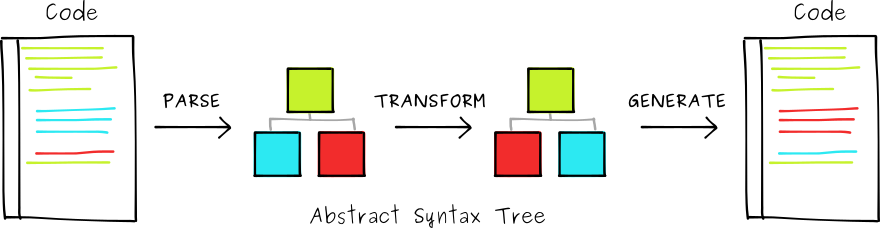
\includegraphics[width=\textwidth]{ast.png}
    \caption{Zasada działania tarnspilatora Babel https://blog.logrocket.com/wp-content/uploads/2020/06/ast.png}
    \label{fig:ast}
\end{figure}

Dlatego właśnie mimo tego, że JavaScript nie jest kompilowany, to jednak istnieje proces buildu, który przygotowuje kod do wdrożenia. Proces ten nazywany jest \textbf{transpilacją}. Babel nie jest obecnie szybkim transpilatorem. Swoją popularność zawdzięcza czasom, w których był jedynym rozwiązaniem na rynku.

Dosyć niedawno spopularyzowanym narzędziem jest SWC. Produkt zajmujący się transpilacją oraz \textbf{bundlowaniem} kodu JavaScriptowego. Obiecuje 20 krotne zwiększenie wydajności na jednym rdzeniu oraz aż 70 krotne zwiększenie wydajności w środowisku 4 rdzeniowym.

Produkty związane z JavaScript adaptują swoje środowiska tak, by korzystanie z SWC było proste. NestJS udostępnia plik konfiguracyjny, w którym dodanie transpilatora SWC sprowadza się do dodania:

\begin{lstlisting}[caption=Fragment pliku konfiguracyjnego nest-cli.json]
"compilerOptions": {
  "builder": "swc"
}
\end{lstlisting}

Zmierzę teraz czas budowania kodu porównując domyślny transpilator (Babel) oraz SWC. W każdym wypadku powtórzę proces 5 razy i wyciągnę średnią korzystając z
\begin{lstlisting}[caption=Komenda mierząca czas wykonania komendy w systemie Windows]
PS >> Measure-Command { start-process npm 'run build' -wait}
\end{lstlisting}


Dodatkowo projekt sztucznie powiększę, aby zasymulować, jak zachowają się obydwa transpilatory przy bardziej złożonych projektach. Poniższe zestawienia przedstawiają porównanie wyników czasu transpilacji.

\begin{table}[H]
\centering
\begin{tabular}{|l|l|l|}
\hline
\textbf{Konfiguracja} & \textbf{Transpilator} & \textbf{Czas wykonania (ms)} \\ \hline
\multirow{2}{*}{60 linijek kodu} & Babel & 5,018 \\ 
& SWC & 4,022 \\ \hline
\multirow{2}{*}{3,000 linijek kodu} & Babel & 24,333 \\ 
& SWC & 8,078 \\ \hline
\multirow{2}{*}{10,000 linijek kodu} & Babel & 29,282 \\ 
& SWC & 9,100 \\ \hline
\end{tabular}
\caption{Czas transpilacji dla różnych konfiguracji}
\label{tab:czas_wykonania}
\end{table}

Oszczędność czasu SWC mimo że przy małym projekcie jest niska, to jednak widoczna. Prawdziwą wyższość SWC widać, gdy w projekcie rośnie liczba linijek kodu. Mimo że obiecana poprawa wydajności w tym wypadku nie została osiągnięta (20 krotne przyspieszenie), na poniższym wykresie zestawiłem te czasy, aby pokazać, że widoczna zależność wskazuje na to, że obiecywana optymalizacja jest jak najbardziej osiągalna przy większej liczbie linijek kodu.

\begin{center}
    \begin{tikzpicture}
    \begin{axis}[
        xlabel={Liczba linijek kodu},
        ylabel={Czas budowy (ms)},
        title={},
        legend pos=north west,
        grid style=dashed,
        xtick={60, 3000, 10000}, % Specify tick marks on the x-axis
        ytick={0, 5000, 25000}, % Specify tick marks on the y-axis
        xticklabels={60, 3000, 10000}, % Labels for the x-axis ticks
        yticklabels={0, 5000, 25000}, % Labels for the y-axis ticks
        scaled y ticks=false, % Disable automatic scaling of y ticks
        ymin=0,
        scaled x ticks=false,
    ]
     
    \addplot[
        color=blue,
        mark=*,
        ]
        coordinates {
        (60, 5018)(3000, 24333)(10000, 29282)
    };
        \addlegendentry{Babel}
    
    \addplot[
        color=red,
        mark=*,
        ]
        coordinates {
        (60, 4022)(3000, 8078)(10000, 9100)
        };
        \addlegendentry{SWC}
    \end{axis}
    \end{tikzpicture}
\end{center} 

\subsection{Frontend}

Jako framework frontendowy wybrałem \textbf{ReactJS}. Tutaj znowu skupię się na początkowej, domyślnej konfiguracji. Narzędziem polecanym przez oficjalną dokumentację React nadal jest CRA (Create React App). Mimo bardzo dużej popularności nie jest to narzędzie optymalne.

U podstawy CRA stoi Webpack, który jest całkiem wolny, ponieważ w momencie procesu budowania musi dokonać zbundlowania wszystkich assetów aplikacji w statyczne pliki.

\begin{figure}[H]
    \centering
    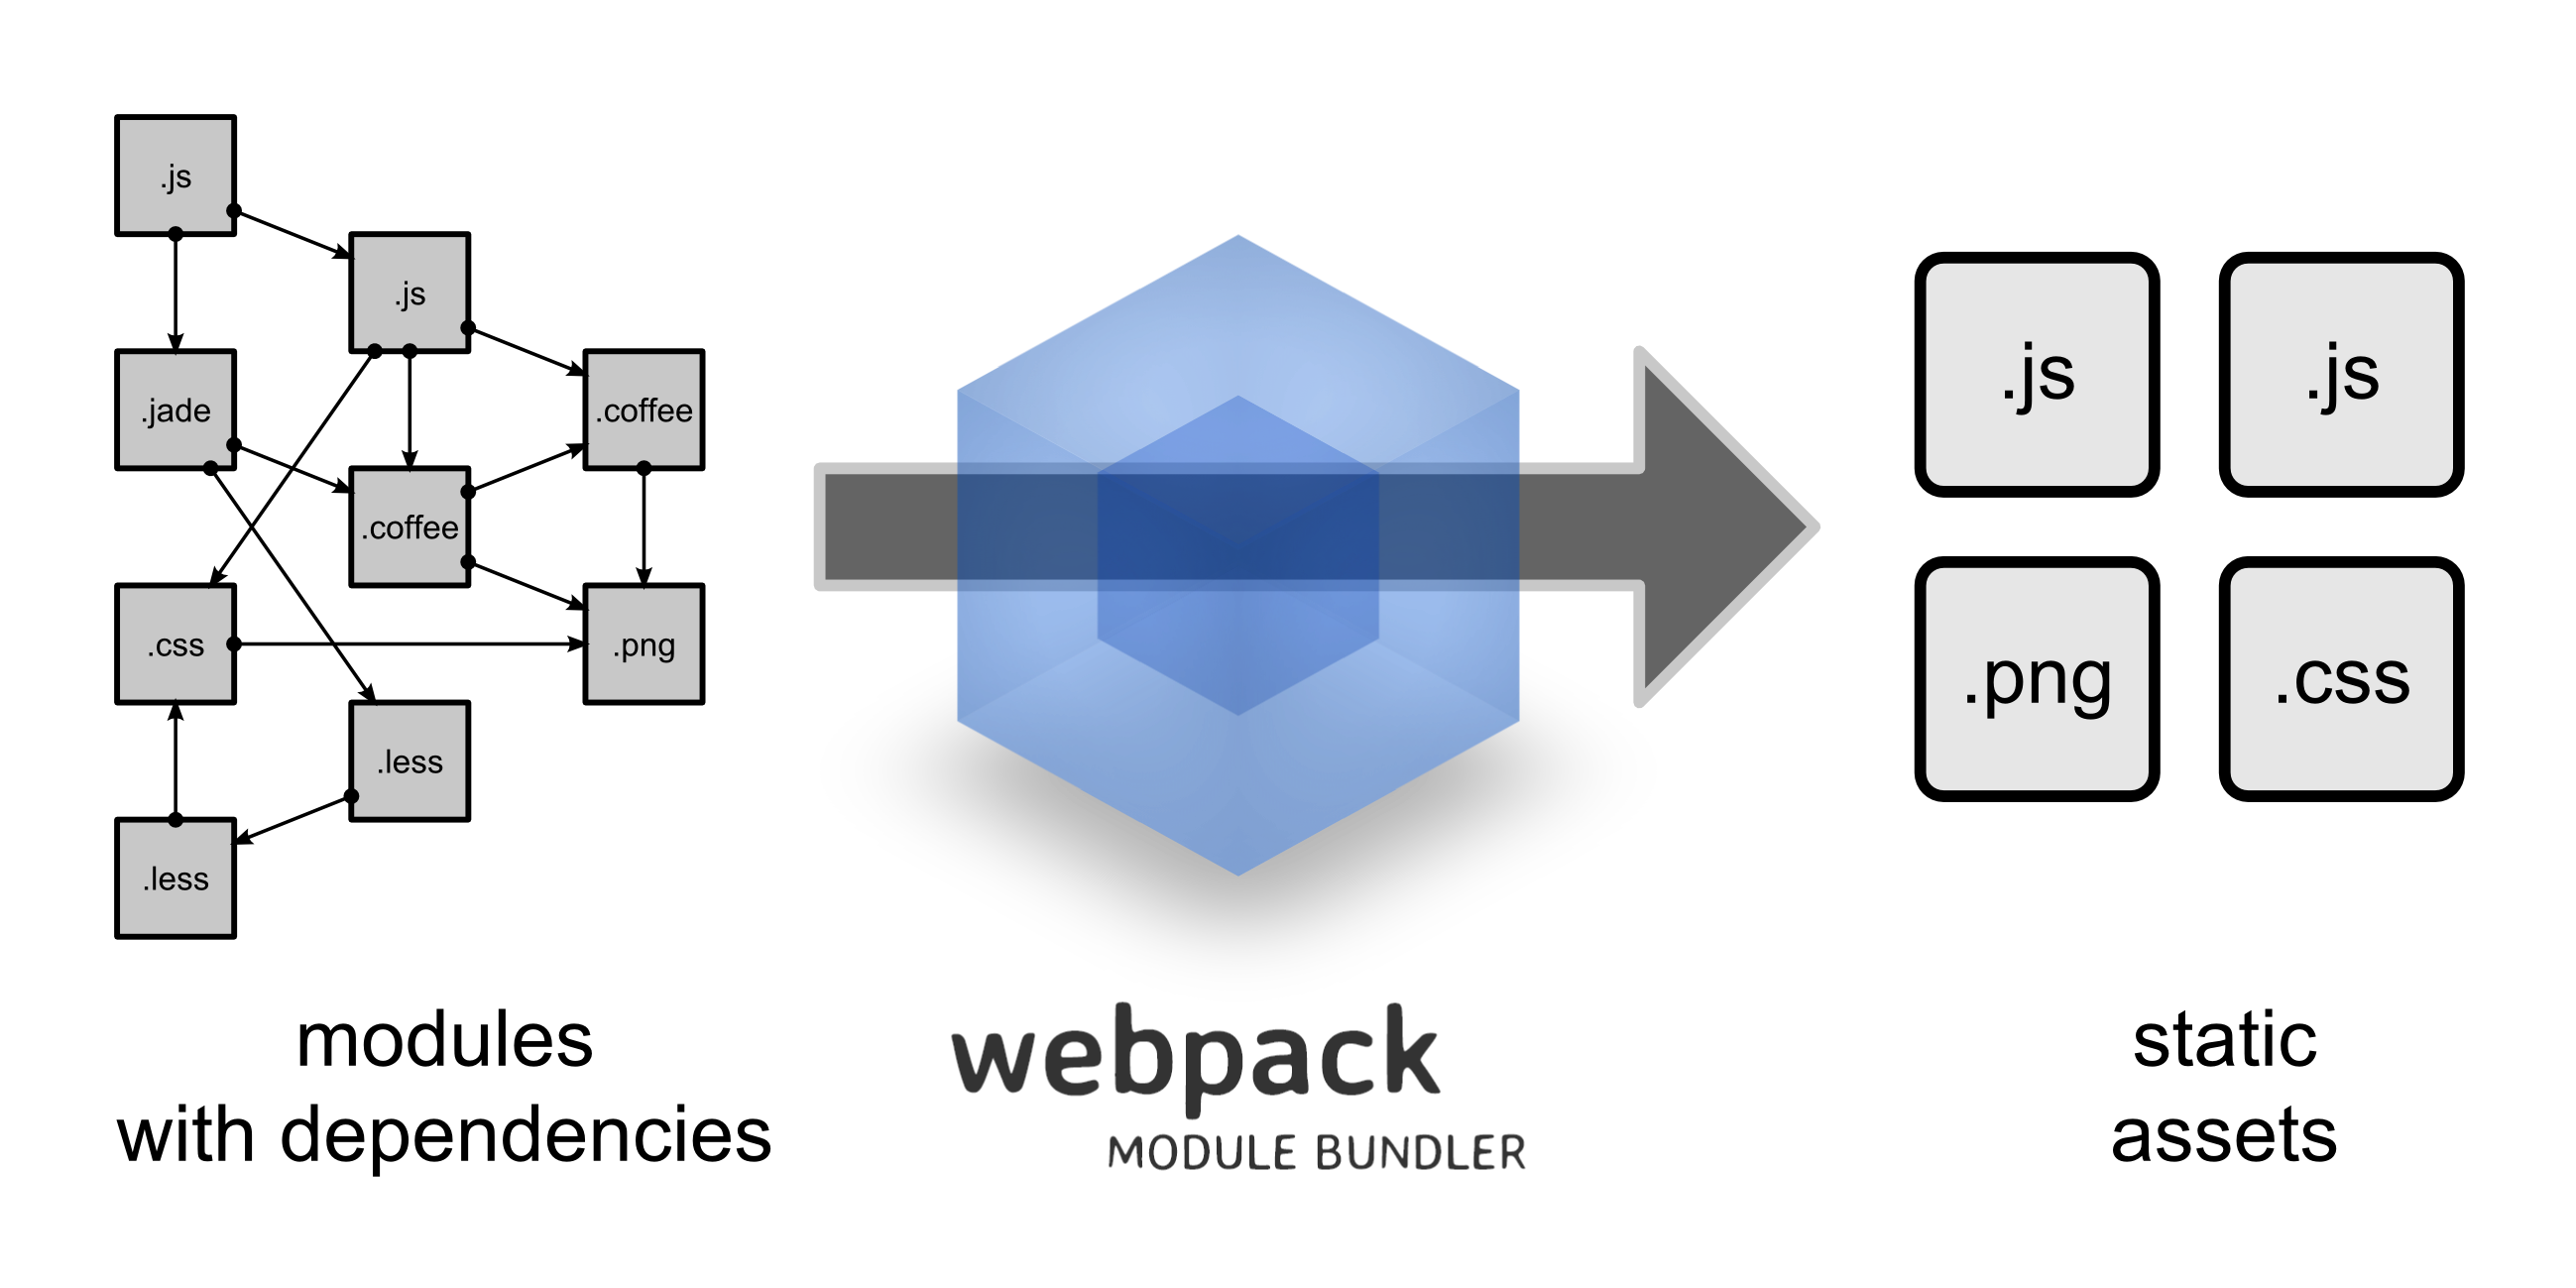
\includegraphics[width=\textwidth]{webpack.png}
    \caption{Zasada działania bundlera Webpack https://camo.githubusercontent.com/eac23581690c3ed7f73c0682aca8362fc0eff51ccd2700d28733f58936dd99d7/68747470733a2f2f7765627061636b2e6769746875622e696f2f6173736574732f776861742d69732d7765627061636b2e706e67}
    \label{fig:ast}
\end{figure}

W dużym projekcie proces ten potrafi być bardzo wolny. Razem z rozwojem ekosystemu JavaScript powstała opcja dynamicznych modułów ESM. Projektem realizującym ten mechanizm jest Vite. Dostarcza on rozwiązanie pozwalające budować i uruchamiać aplikacje Reactowe o wiele szybciej. Sprawa on, że kod, który aktualnie nie musi być używany, nie jest załadowany do pamięci - jest ładowany dynamicznie. Zasadniczym plusem takiego rozwiązania jest wsparcie dla HMR (Hot Module Reload) dzięki któremu w środowisku deweloperskim po wprowadzeniu drobnej zmiany nie jest konieczne ponowne zbundlowanie całego projektu, a tylko podmiana niewielkiego fragmentu kodu.

W tej części porównam czasy włączenia serwera deweloperskiego oraz zbudowania aplikacji.

Aplikację korzystającą z CRA stworzyłem korzystając z następujących komend:

\begin{lstlisting}[caption=Stworzenie i włączenie aplikacji React (CRA)]
npx create-react-app frontend-cra
cd frontend-cra
npm run start
\end{lstlisting}

Aplikację korzystającą z Vite stworzyłem używając: 

\begin{lstlisting}[caption=Stworzenie i włączenie aplikacji React (CRA)]
npm create vite@latest frontend-vite -- --template react-ts
cd frontend-vite
npm run dev
\end{lstlisting}

Obydwie aplikacje mają około 200 linijek kodu na starcie. W celu badania w drugim kroku rozszerzyłem je do około 10,000 linijek kodu. Poniższa zestawienie prezentuje czasy wykonywania poszczególnych operacji.

\begin{table}[H]
\centering
\begin{tabular}{|l|l|l|}
\hline
\textbf{Operacja} & \textbf{Liczba linijek} & \textbf{Czas wykonania (s)} \\ \hline
\multirow{2}{*}{Włączenia serwera deweloperskieogo} & 200 & 10 \\ 
& 10,000 & 39 \\ \hline
\multirow{2}{*}{Zbudowanie aplikacji} & 200 & 19 \\ 
& 10,000 & 50 \\ \hline
\end{tabular}
\caption{Czasy operacji dla CRA}
\label{tab:czas_wykonania}
\end{table}

\begin{table}[H]
\centering
\begin{tabular}{|l|l|l|}
\hline
\textbf{Operacja} & \textbf{Liczba linijek} & \textbf{Czas wykonania (s)} \\ \hline
\multirow{2}{*}{Włączenia serwera deweloperskieogo} & 200 & 2 \\ 
& 10,000 & 3 \\ \hline
\multirow{2}{*}{Zbudowanie aplikacji} & 200 & 5 \\ 
& 10,000 & 8 \\ \hline
\end{tabular}
\caption{Czasy operacji dla Vite}
\label{tab:czas_wykonania}
\end{table}


Poniżej czasy zestawione na wykresie:


\begin{figure}[H]
\centering
\begin{tikzpicture}
\begin{axis}[
    title={Porównanie czasów operacji dla CRA i Vite},
    xlabel={Liczba linijek},
    ylabel={Czas wykonania (s)},
    xmin=0, xmax=10500,
    ymin=0, ymax=55,
    xtick={200,10000},
    ytick={0,10,20,30,40,50},
    legend pos=north west,
    ymajorgrids=true,
    grid style=dashed,
    scaled y ticks=false,
    scaled x ticks=false,
]

\addplot[
    color=blue,
    mark=square,
    ]
    coordinates {
    (200,10)(10000,39)
    };
\addlegendentry{CRA - Włączenie serwera}

\addplot[
    color=blue,
    mark=triangle,
    ]
    coordinates {
    (200,19)(10000,50)
    };
\addlegendentry{CRA - Zbudowanie aplikacji}

\addplot[
    color=red,
    mark=square,
    ]
    coordinates {
    (200,2)(10000,3)
    };
\addlegendentry{Vite - Włączenie serwera}

\addplot[
    color=red,
    mark=triangle,
    ]
    coordinates {
    (200,5)(10000,8)
    };
\addlegendentry{Vite - Zbudowanie aplikacji}

\end{axis}
\end{tikzpicture}
\caption{Porównanie czasów operacji dla CRA i Vite}
\label{fig:cra_vs_vite}
\end{figure}

Jak widać, Vite oferuje niewiarygodne przyspieszenie czasu budowania. Co zdumiewające, nachylenie funkcji czasu wykonywania od liczby linijek jest bardzo niewielkie, co powoduje, że czym większy projekt, tym ta oszczędność staje się większa.

\subsection{Podsumowanie}

Powyższe badania udowadniają, że często domyślne zestawy narzędzi są dalekie od optymalnych. Optymalizację devops warto zacząć już od samego dobrania narzędzi najlepiej jeszcze przed rozpoczęciem projektu. Zmiany rozmiaru tych opisanych w powyższym rozdziale mogą być bardzo kosztowne w późniejszych fazach projektu.

\section{Metody wdrażania}

Po zbudowaniu aplikacji trzeba jej kod w jakiś sposób przenieść na serwer i na nim włączyć. Wypiszę teraz zarys sposobów, a w następnych działach każdy z nich opiszę dokładniej:

\begin{itemize}
    \item całkowicie ręczne wdrażanie na serwer - deweloper dostaje się na serwer, pobiera kod, instaluje potrzebne zależności i włącza na nim aplikację,
    \item ręczne wdrażanie z dodatkiem - deweloper nadal robi wszystko ręcznie, ale nad działaniem aplikacji czuwa pewien framework. Np. \textbf{Nodemon} do aplikacji NodeJS,
    \item manualna wirtualizacja - deweloper samodzielnie buduje obraz i wysyła go do repozytorium artefaktów. Następnie dostaje się do serwera i tam włącza obraz,
    \item automatyczna wirtuzalicja - istnieje proces, który po wprowadzeniu zmian automatycznie buduje obraz i wdraża go na serwer.
\end{itemize}

Wszystkie powyższe techniki zakładają, że deweloper ma dostęp do serwera poprzez SSH, a sam serwer jest uwierzytelniony do repozytorium kodu.

\subsection{Całkowicie ręczne wdrażanie}

Deweloper włącza manualnie aplikacje na serwerze. Musi podjąć większość kroków wykonywanych w środowisku lokalnym plus upewnić się, że serwer poprawnie obsługuje zapytania przychodzące z zewnątrz.

Szczególnie uciążliwa może być pierwsza konfiguracja. Należy w jej obrębie pobrać i skonfigurować narzędzia potrzebne do budowania i wdrażania aplikacji w danej technologii. W przypadku NodeJS będzie to npm. Dodatkowo może się okazać, że niektóre z zależności potrzebnych do działania aplikacji były zainstalowane globalnie na komputerze dewelopera, co spowoduje, że aplikacja nie zadziała i przysporzy to problemów natury debugowania.

\begin{figure}[H]
    \centering
    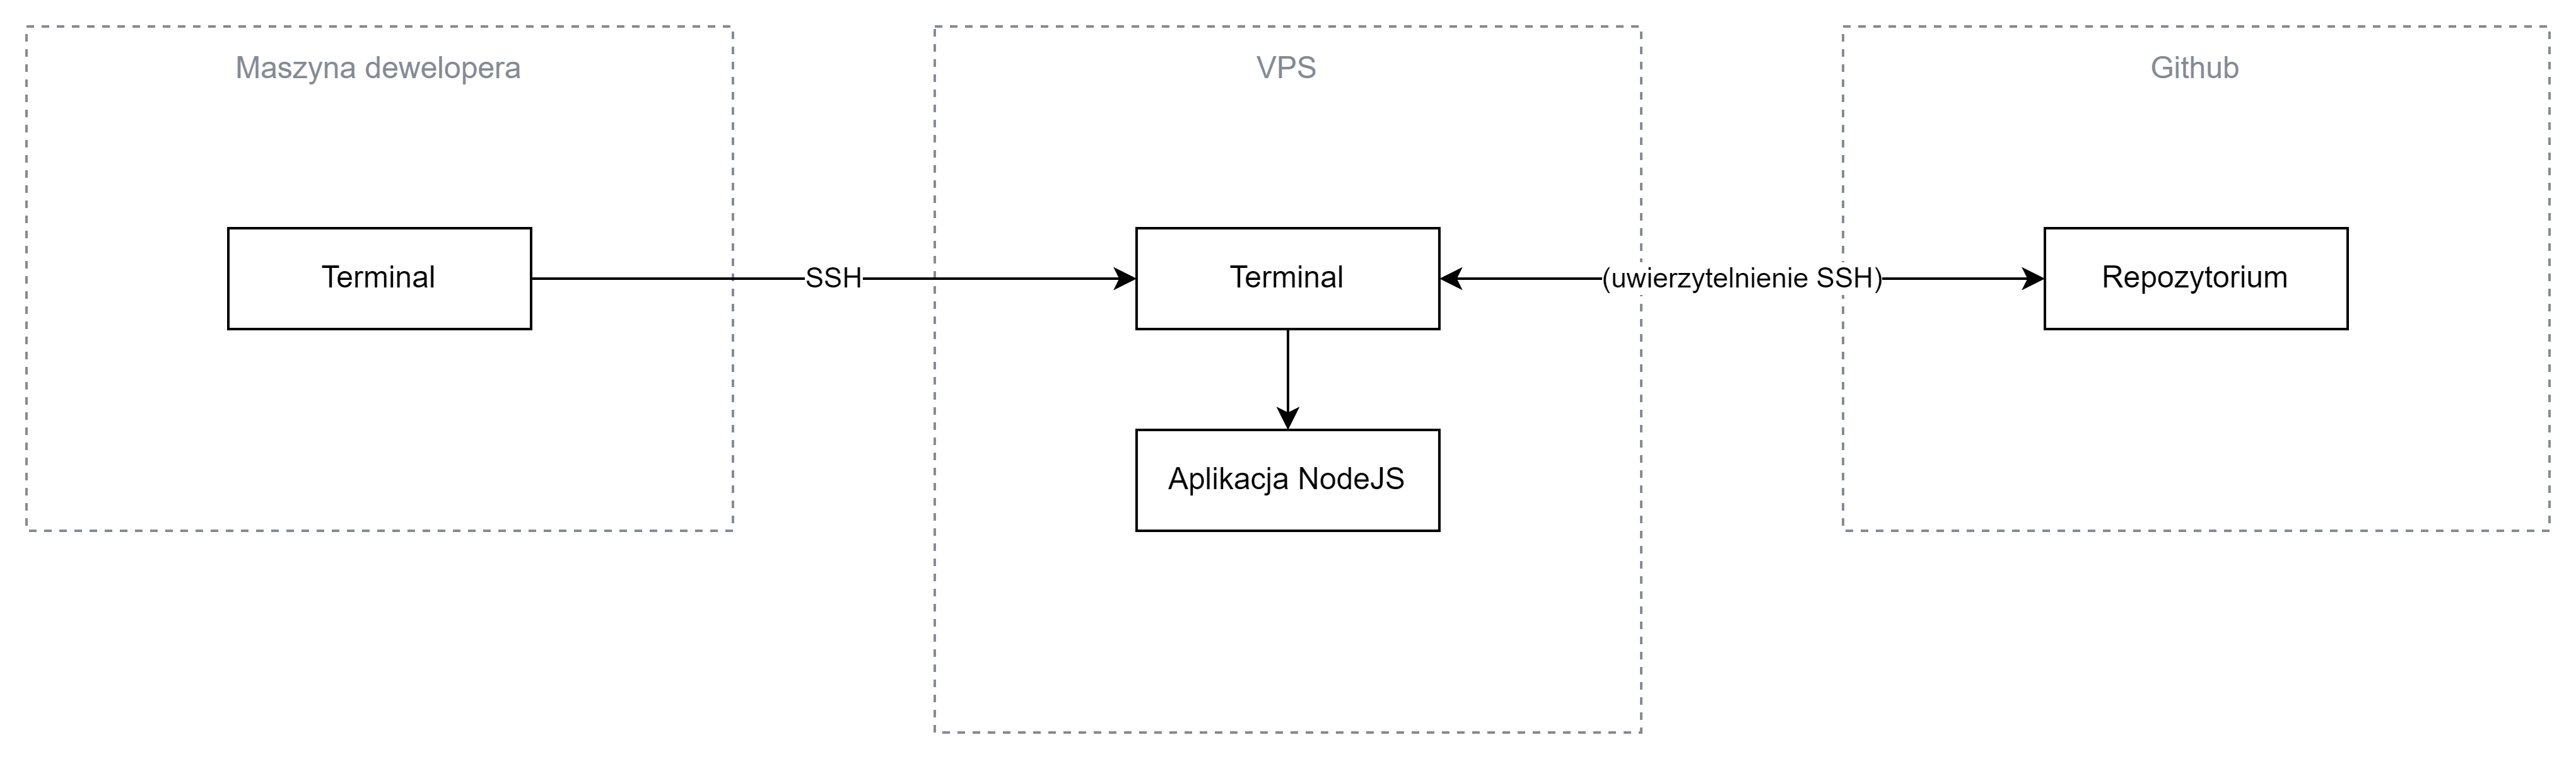
\includegraphics[width=1\linewidth]{reczne_wdrazanie.png}
    \caption{Całkowicie ręczne wdrażanie}
    \label{fig:enter-label}
\end{figure}

\begin{itemize}
    \item pobranie nowej wersji kodu,
    \item zainstalowanie potrzebnych zależności,
    \item zatrzymanie starej wersji aplikacji,
    \item włączenie nowej wersji aplikacji
\end{itemize}

\subsubsection{Zalety}

Metoda ta ma tylko jedną zaletę - czas. Pierwsze wdrożenie na serwer odbędzie się z pewnością szybciej. Nie ma potrzeby konfiguracji narzędzi automatyzujących pracę.

\subsubsection{Wady}

\begin{itemize}
    \item tracenie czasu na bardzo powtarzalne czynności przy każdym wdrożeniu,
    \item możliwość, że aplikacja nie będzie działać z uwagi na różnice w konfiguracji środowiska,
    \item brak możliwości dobrego monitorowania aplikacji,
    \item brak zarządzania stanem aplikacji (po restarcie serwera lub krytycznym błędzie w aplikacji pozostanie ona wyłączona),
    \item aplikacja ma bezpośredni dostęp do systemu operacyjnego hosta.
\end{itemize}

\subsection{Ręczne wdrażanie z dodatkiem}

Jako dodatek do ręcznego wdrożenia wybrałem Nodemon. Jest to narzędzie wprowadzające warstwę abstrakcji na aplikację NodeJS. Jest w stanie zarządzać stanem aplikacji - monitoruje, czy aplikacja jest "zdrowa". Dodatkowo pozwala na skalowanie aplikacji i zapewnia automatyczny load balancing. 

\begin{figure}[H]
    \centering
    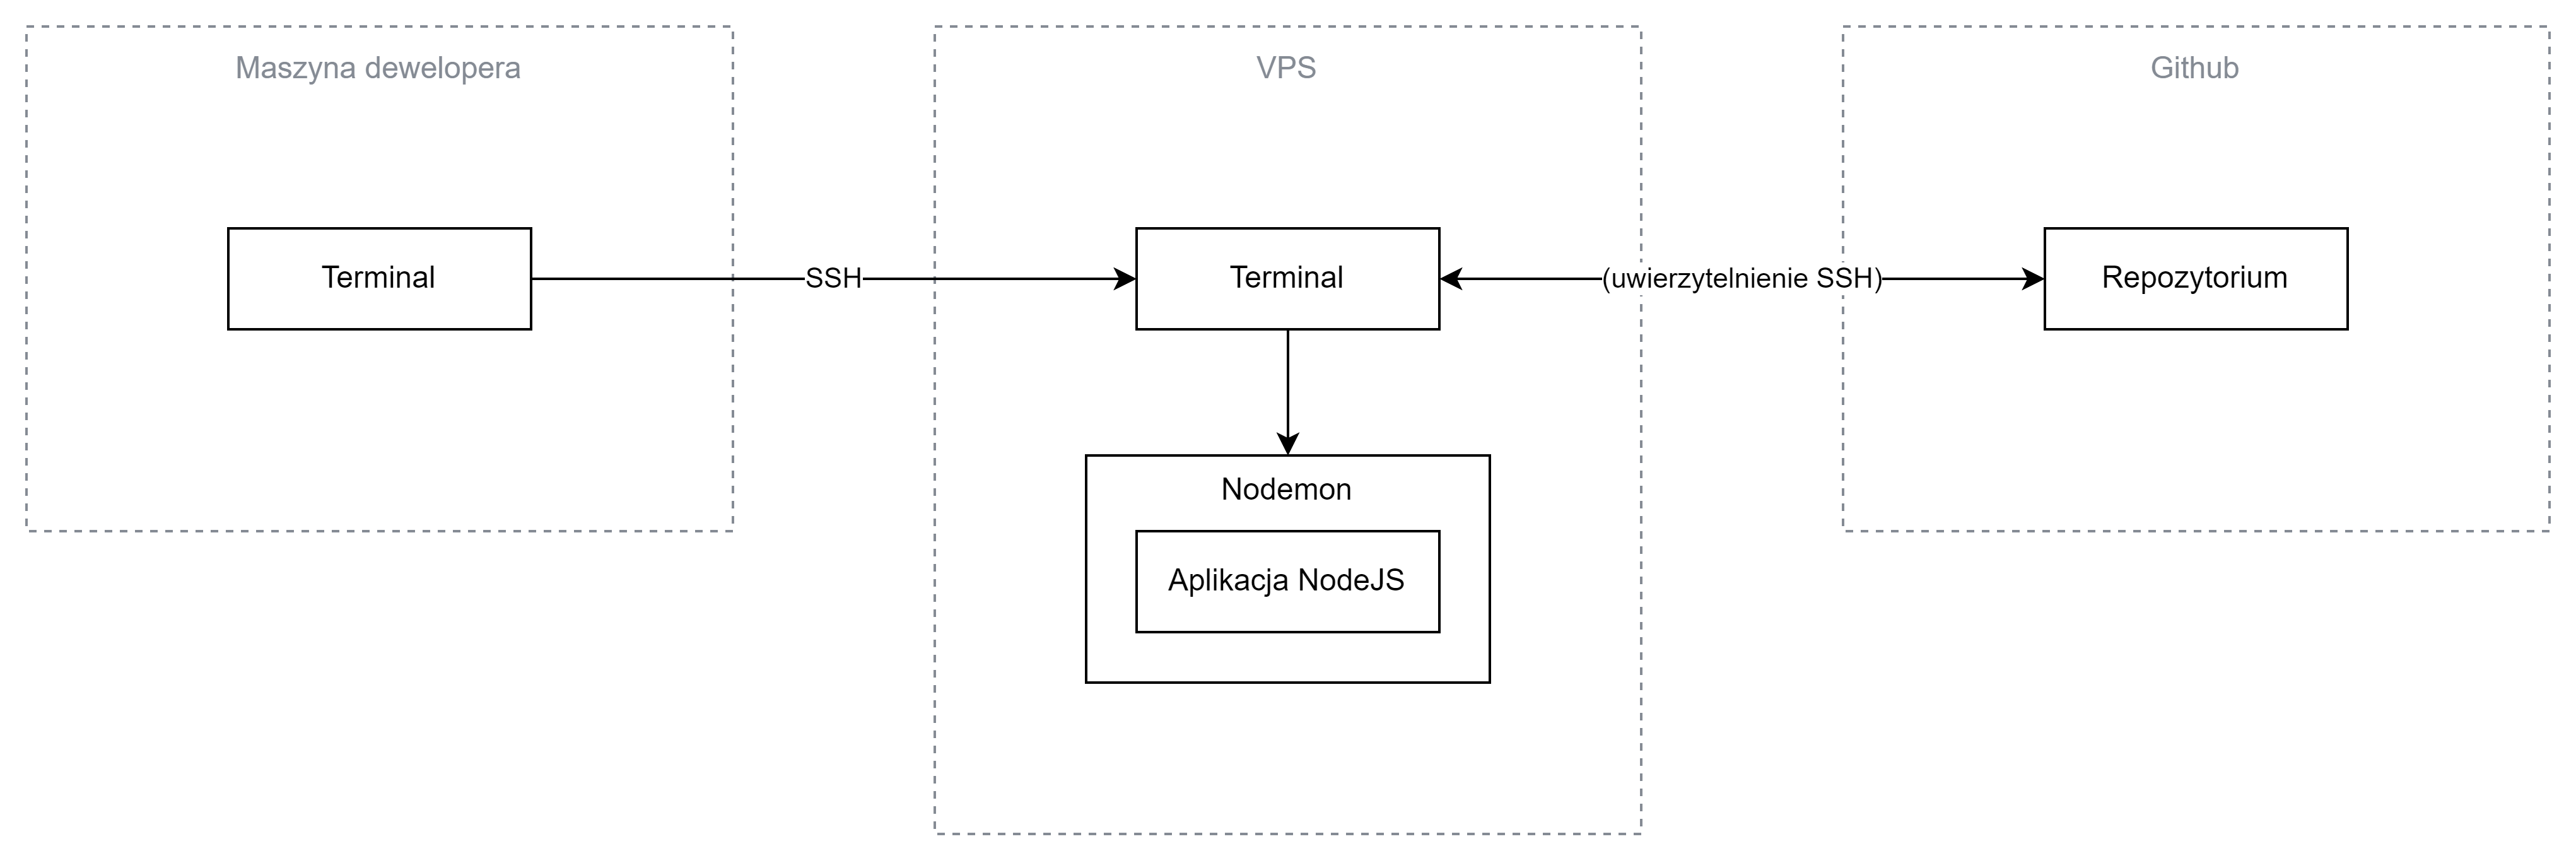
\includegraphics[width=1\linewidth]{reczneWdrazanieZDodatkiem.png}
    \caption{Ręczne wdrażanie z dodatkiem}
    \label{fig:enter-label}
\end{figure}

\subsubsection{Zalety}

\begin{itemize}
    \item podstawowe możliwości monitorowania aplikacji,
    \item zarządzanie stanem aplikacji (aplkacja sama się restartuje, jeżeli jest taka potrzeba),
    \item udostępnienie interfejsu do prostego skalowania aplikacji oraz automatycznego load balancera.
\end{itemize}

\subsubsection{Wady}

\begin{itemize}
    \item aplikacja nadal narażona jest na różnice w konfiguracji środowiska,
    \item aplikacja nadal ma bezpośredni dostęp do systemu operacyjnego hosta.
\end{itemize}

\subsection{Manualna wirtualizacja}

W tym przypadku deweloper buduje manualnie obraz na swoim komputerze i wysyła go do repozytorium artefaktów. Następnie dostaje się do maszyny, pobiera na niej obraz i włącza kontener z nową wersją aplikacji.

\begin{figure}[H]
    \centering
    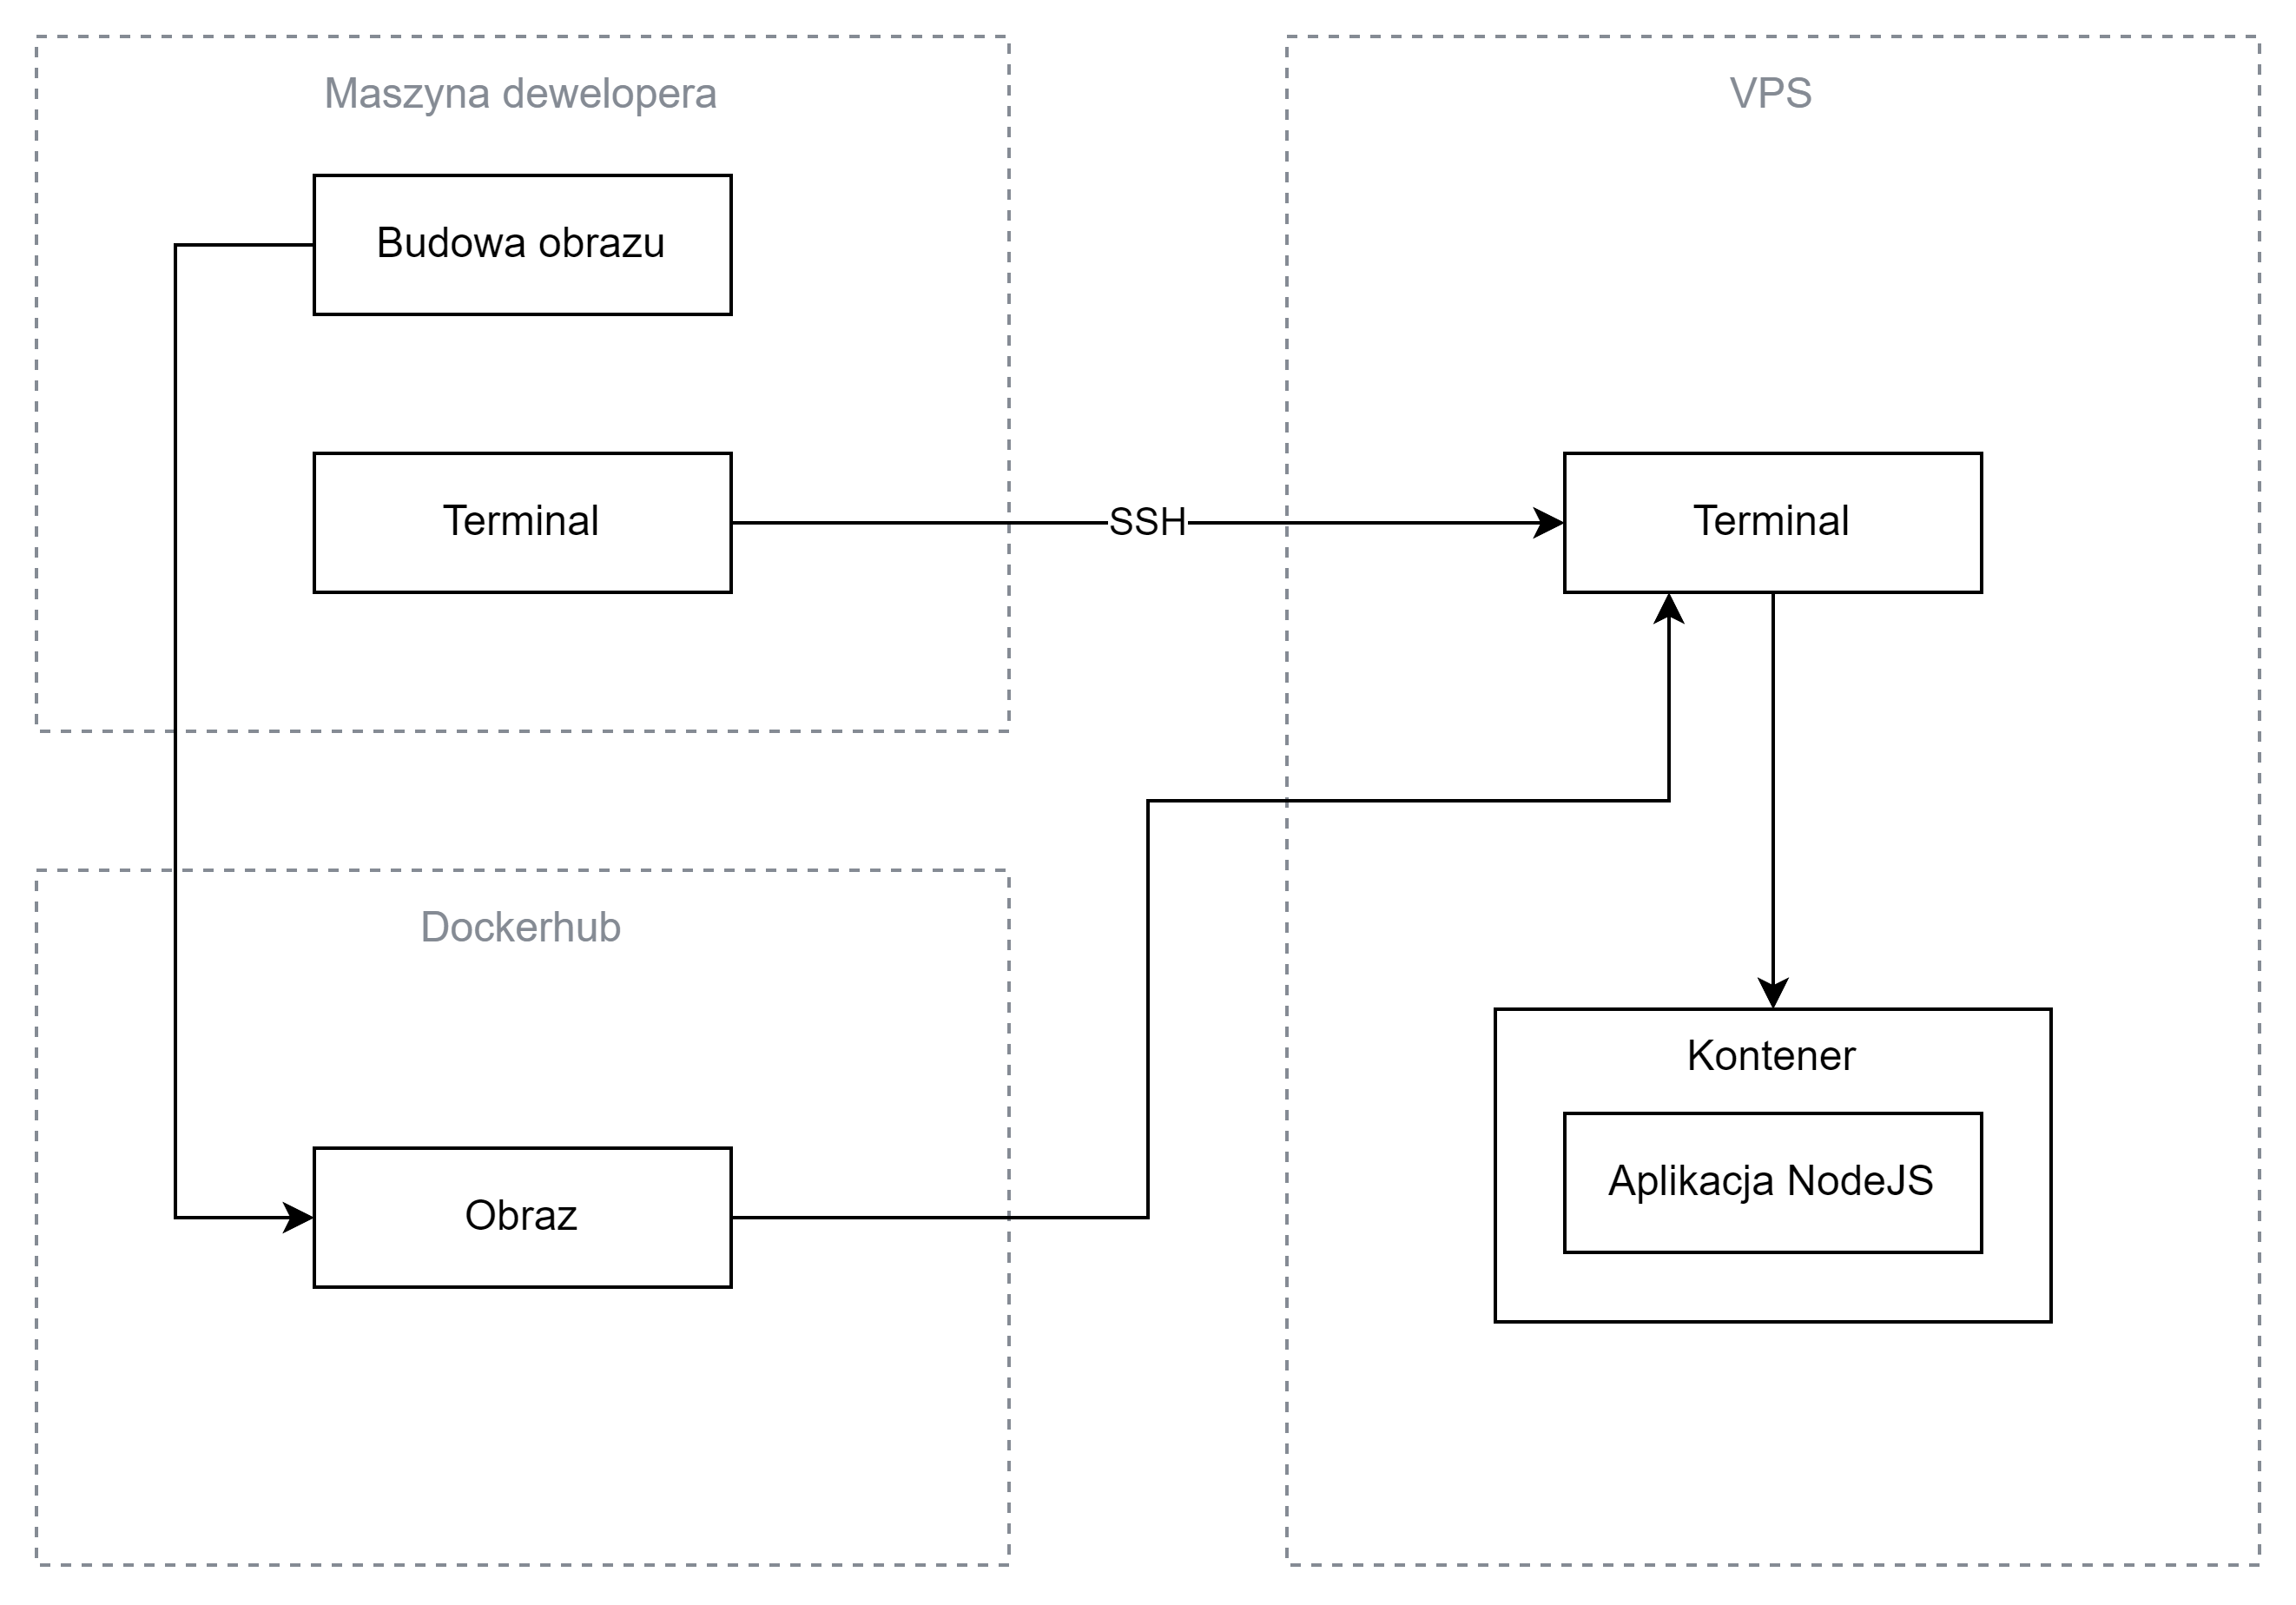
\includegraphics[width=1\linewidth]{manualnaWirtualizacja.png}
    \caption{Manualna wirtualizacja}
    \label{fig:enter-label}
\end{figure}

\subsubsection{Zalety}

\begin{itemize}
    \item o wiele szybsza konfiguracja środowiska. Na serwerze musi być tylko zainstalowany narzędzie obsługujące wirtualizację,
    \item drastycznie zredukowana szansa wystąpienia błędów w wyniku różnic w konfiguracji. Deweloper może obraz najpierw przetestować na swojej lokalnej maszynie,
    \item aplikacja nie ma dostępu do systemu operacyjnego hosta.
\end{itemize}

\subsubsection{Wady}

\begin{itemize}
    \item znaczne skomplikowanie infrastruktury projektu. Od teraz trzeba utrzymywać repozytorium obrazów,
    \item utrudnienie zmian w konfiguracji aplikacji. Możliwe, że zwykły deweloper nie będzie potrafił wprowadzić zmian obejmujących rzeczy poza samym kodem do aplikacji,
\end{itemize}

\subsection{Wirtualizacja + CI/CD}

W tym podejściu deweloper buduje infrastrukturę CI/CD umożliwiając całkowicie automatyczne wdrażanie aplikacji. Po wgraniu do repozytorium kodu zmian, agent automatycznie się uruchamia, buduje obraz, a następnie dostaje się do serwera i na nim włącza kontener

\begin{figure}[H]
    \centering
    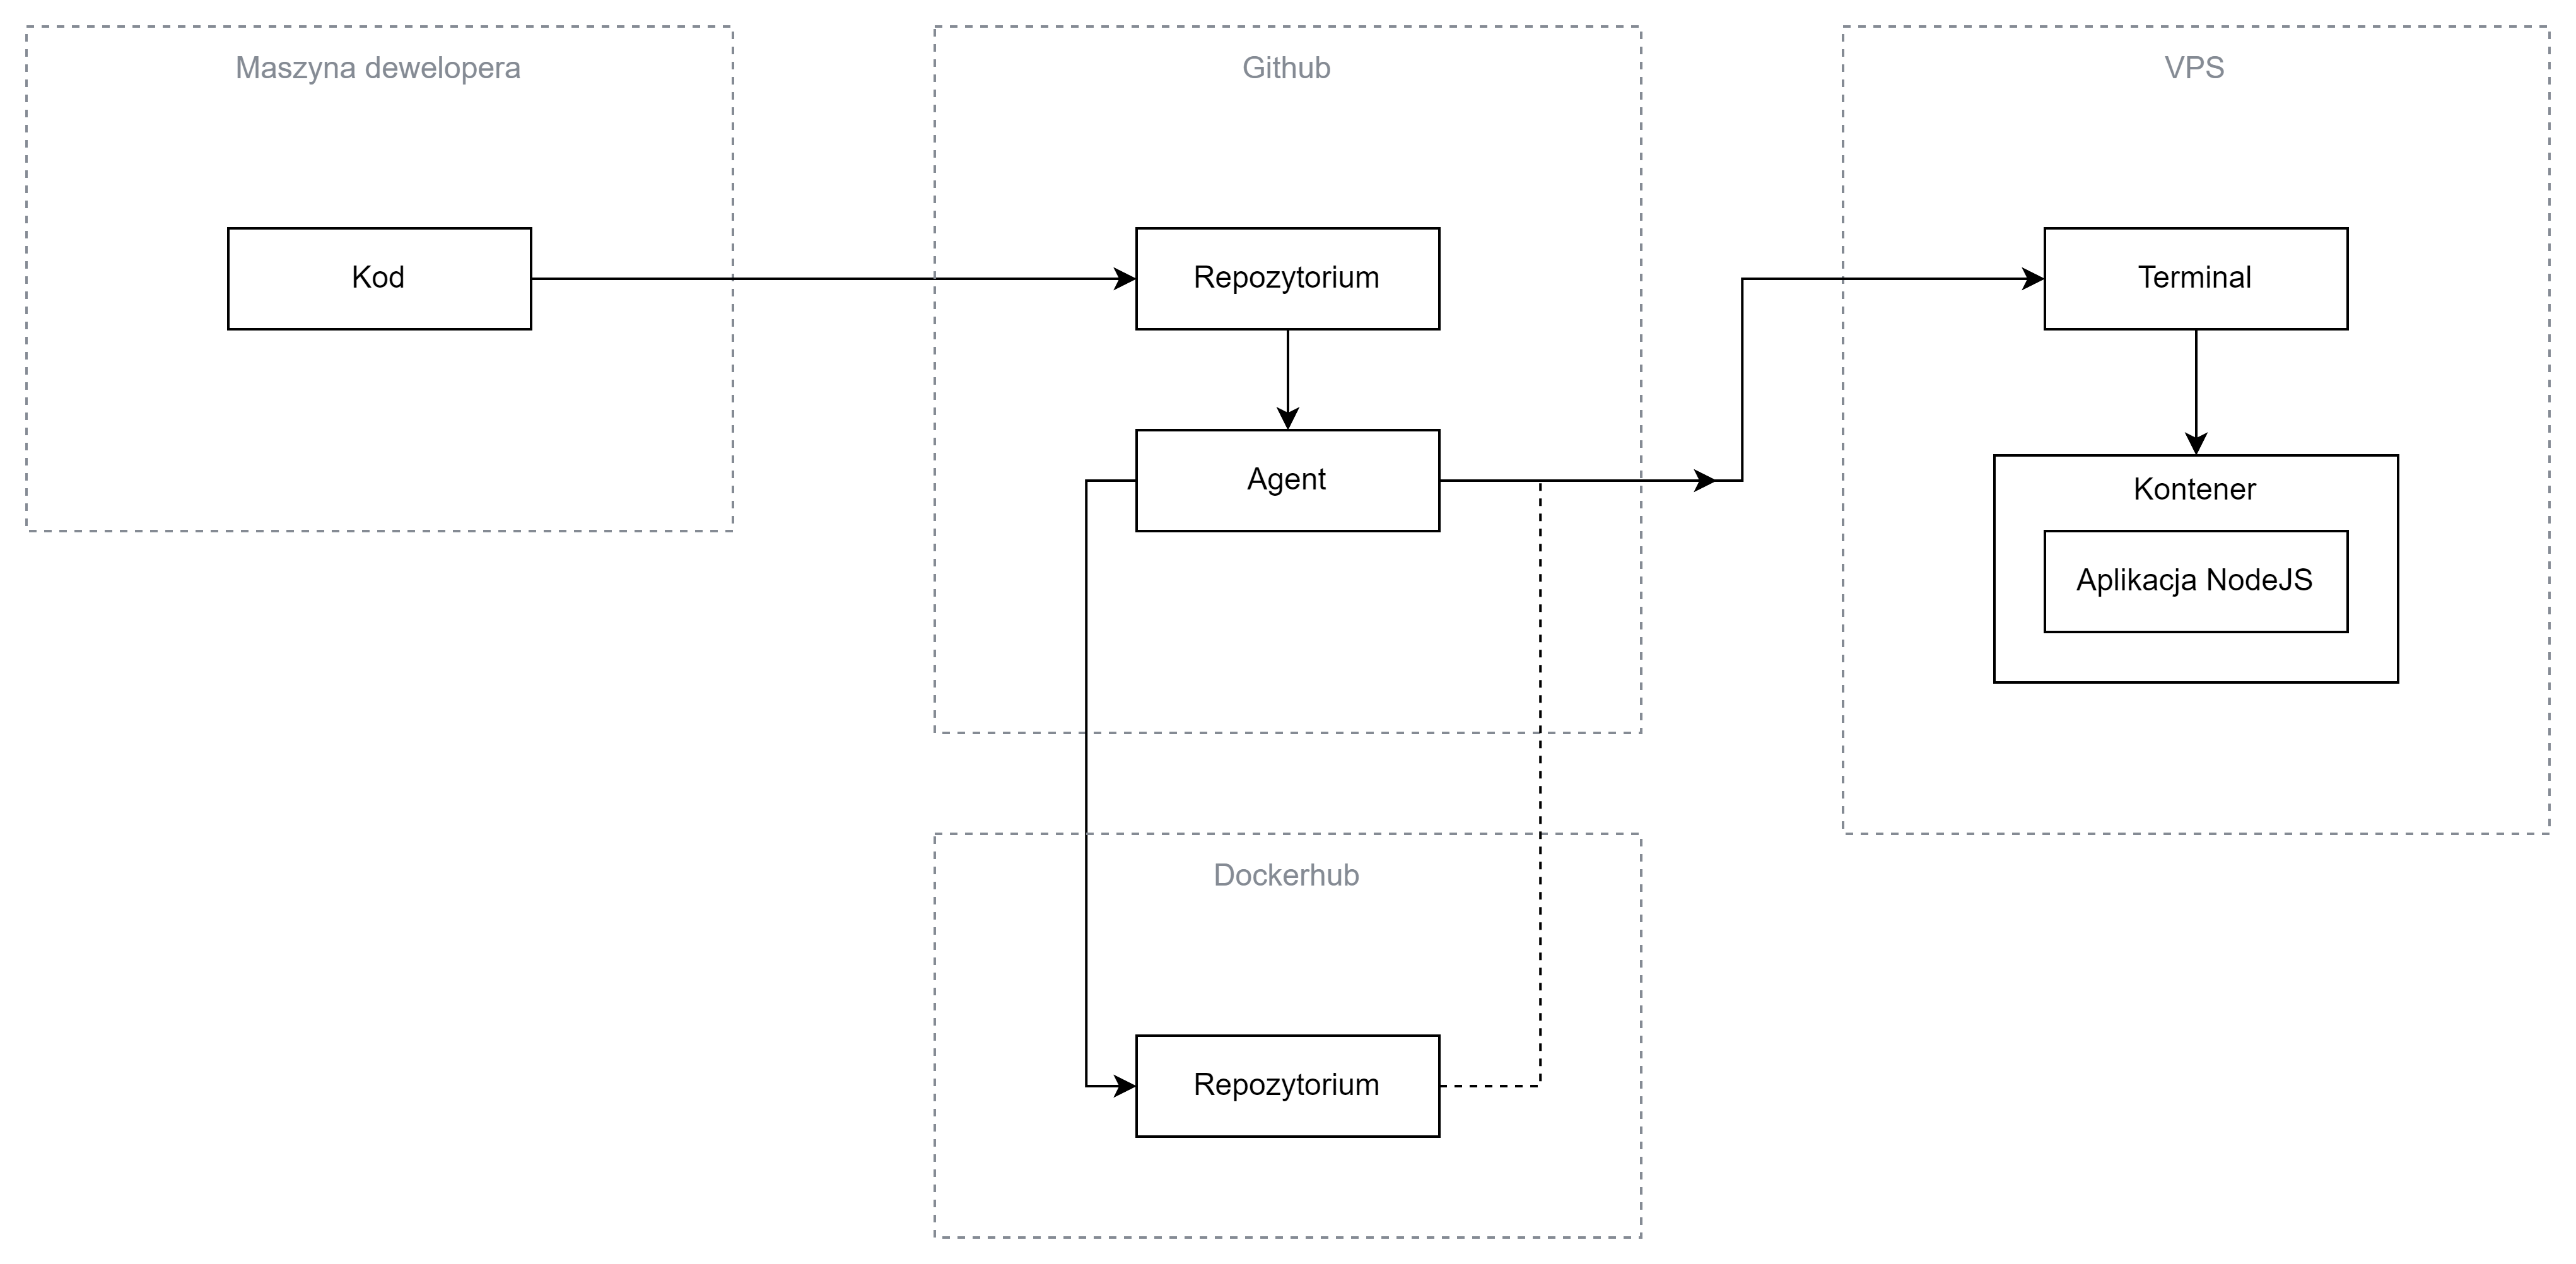
\includegraphics[width=1\linewidth]{automatycznaWirtualizacja.png}
    \caption{Wirtualizacja + CI/CD}
    \label{fig:enter-label}
\end{figure}

\subsubsection{Zalety}

\begin{itemize}
    \item znaczące usprawnienie procesu wdrażania aplikacji,
    \item minimalizacja błędów konfiguracji,
    \item bardzo łatwe rozszerzenie na kilka środowisk.
\end{itemize}

\subsubsection{Wady}

\begin{itemize}
    \item znaczne skomplikowanie infrastruktury projektu. Potrzeba wybrania narzędzia do CI/CD oraz tworzenia i utrzymywania plików konfiguracyjnych,
\end{itemize}

\subsection{Podsumowanie}

\begin{table}[H]
\centering
\begin{tabular}{|l|c|c|c|c|}
\hline
\textbf{Cecha} & \textbf{1} & \textbf{2} & \textbf{3} & \textbf{4} \\ \hline
Podatność na błędy konfiguracji         & \cellcolor{red!50}wysoka & \cellcolor{red!50}wysoka & \cellcolor{green!50}niska & \cellcolor{green!50}niska \\ \hline
Czas potrzebny na pierwszą konfigurację & \cellcolor{green!50}niski & \cellcolor{yellow!50}średni & \cellcolor{red!50}wysoki & \cellcolor{red!50}bardzo wysoki \\ \hline
Czas wdrożenia nowej wersji aplikacji   & \cellcolor{red!50}wysoki & \cellcolor{red!50}wysoki & \cellcolor{yellow!50}średni & \cellcolor{green!50}niski \\ \hline
Zarządzanie stanem aplikacji            & \cellcolor{red!50}nie & \cellcolor{green!50}tak & \cellcolor{green!50}tak & \cellcolor{green!50}tak \\ \hline
Skalowanie aplikacji                    & \cellcolor{red!50}trudne & \cellcolor{green!50}łatwe & \cellcolor{green!50}łatwe & \cellcolor{green!50}łatwe \\ \hline
Podatność na ataki                      & \cellcolor{red!50}wysoka & \cellcolor{red!50}wysoka & \cellcolor{green!50}niska & \cellcolor{green!50}niska \\ \hline
Monitorowanie aplikacji                 & \cellcolor{red!50}nie & \cellcolor{red!50}nie & \cellcolor{green!50}tak & \cellcolor{green!50}tak \\ \hline
\end{tabular}
\caption{Porównanie metod wdrażania: 1 - całkowicie ręczne, 2 - ręczne z dodatkiem, 3 - wirtualizacja, 4 - wirtualizacja + CI/CD}
\label{tab:porownanie-metod-wdrazania}
\end{table}

Zasadniczym plusem ręcznego wdrażania jest szybkość pierwszej konfiguracji. Nie trzeba konfigurować praktycznie nic, tylko włączyć aplikację na serwerze. Uważam jednak, że liczba zalet wirtualizacji z użyciem CI/CD przewyższa zysk czasowy manualnego wdrażania. Warto poświęcić na początku więcej czasu na dobrą konfigurację aby zaoszczędzić go w późniejszych fazach rozwoju aplikacji.


\section{Budowa obrazu}

\subsection{Podstawowy obraz}

Zacznę od przeanalizowania najprostszego obrazu dockerowego, aby aplikacja po prostu działała. W tym celu dodałem do folderu z aplikacją plik \textbf{Dockerfile} o następującej treści

\begin{lstlisting}[caption=Podstawowy plik Dockerfile]
FROM node:18

WORKDIR /usr/src/app

COPY package*.json ./

RUN npm install

COPY . .

RUN npm run build

CMD [ "node", "dist/main.js" ]
\end{lstlisting}

Z definicji pliku wynika, że wybiera on obraz bazowy, przenosi pliki konfiguracyjne, instaluje potrzebne zależności, przenosi pliki źródłowe, buduje aplikacje i ją włącza.

Czas potrzebny na zbudowanie obrazu to \textbf{85 sekund}. Rozmiar obrazu to \textbf{1.64GB}. Warto zwrócić uwagę na to, który krok zajął najwięcej czasu. Był to krok \lstinline|[internal] load build context|.

\subsection{Dockerignore}

Warto wiedzieć, że NodeJS potrzebne zależności przechowuje w folderze, w którym znajdują się pliki projektu. Oznacza to, że instrukcja \lstinline|COPY . .| z pliku Dockerfile przeniesie je wszystkie do obrazu, co nie jest konieczne, ponieważ w obrazie i tak trzeba je pobrać.

W takim celu używa się pliku \lstinline|.dockerignore|, w którym podaje się listę rzeczy, które Docker ma ignorować podczas instrukcji kopiowania

\begin{lstlisting}[caption=Plik .dockerignore]
dist
node_modules
\end{lstlisting}

Oprocz folderu z zależnościami dobrze nie przenosić również folderu ze zbudowaną aplikacją, ponieważ ta i tak musi się zbudować ponownie w obrazie

Po wprowadzeniu pliku \lstinline|.dockerignore| proces zajmuje teraz \textbf{24 sekundy}, a rozmiar zbudowanego obrazu to \textbf{1.42GB}.

\subsection{Multi stage build}

Node dzieli swoje zależności na standardowe i deweloperskie. Standardowe to te, które są potrzebne do tego, żeby aplikacja działała. Deweloperskie natomiast to takie, które są potrzebne tylko w momencie budowania aplikacji.

Dobrym przykładem zależności deweloperskiej jest \textbf{Typescript}. Jest to paczka, która zawiera definicje potrzebne do przetłumaczenia Typescript na Javascript, ale po przetłumaczeniu nie jest już potrzebna,

\begin{lstlisting}[caption=Multistage plik Dockerfile]
FROM node:18 AS development
WORKDIR /usr/src/app
COPY package*.json ./
RUN npm ci -f
COPY . .


FROM node:18 AS build
WORKDIR /usr/src/app
COPY package*.json ./
COPY --from=development /usr/src/app/node_modules ./node_modules
COPY . .
RUN npm run build
RUN npm ci -f --only=production && npm cache clean --force


FROM node:18 AS production
ENV NODE_ENV production
COPY --from=build /usr/src/app/node_modules ./node_modules
COPY --from=build /usr/src/app/dist ./dist
CMD [ "node", "dist/main.js" ]
\end{lstlisting}

Wylistowany wyżej plik \lstinline|Dockerfile| stosuje 3 etapowy proces budowania.

\begin{enumerate}
    \item development - ta część odpowiedzialna jest za zainstalowanie zależności i skopiowanie plików źródłowych do obrazu,
    \item build - ta część kopiuje zależności, które pobrał pierwszy krok, buduje aplikacje, a następnie wywołuje komendę \lstinline|npm ci -f --only=production && npm cache clean --force|, która nadpisuje zależności w taki sposób, że zostaną tylko te wymagane do poprawnego działania aplikacji (zignoruje zależności deweloperskie,
    \item production - ostatni krok kopiuje potrzebne zależności oraz kod źródłowy i włącza aplikację
\end{enumerate}

Ta konfiguracja zajmuje \textbf{30 sekund}, a rozmiar zbudowanego obrazu to \textbf{1.09GB}

\subsection{Alpine}

Dotychczas korzystałem z obrazu bazowego \lstinline|node:18|. Jest on całkiem spory, ponieważ zawiera pełną dystrubucję linuxa. W przypadku tej (i zdecydowanej większości) aplikacji nie jest potrzebne większość narzędzi z oficjalnej dystrybucji linuxa. 

Można w tym celu użyć dystrybucji typu \textbf{alpine}. Nazwa obrazu to wtedy \lstinline|node:18-alpine|.

W tej konfiguracji obraz buduje się \textbf{33 sekundy} i zajmuje \textbf{148MB} miejsca.

\subsection{Distroless}

Działania opisane w poprzednich krokach miały na celu przyspieszenie procesu budowania lub zmniejszenie rozmiaru obrazu. Istnieje jednak pewna praktyka, którą stosuje się w celu zwiększenie bezpieczeństwa aplikacji.

Sama wirtualizacja zapewnia to, że jeżeli atakujący dostanie się na maszynę, na której włączona jest aplikacja, to nie ma dostępu do systemu operacyjnego hosta, tylko jest "zamknięty" w kontenerze. Ogranicza to znacząco liczbę niechcianych rzeczy, które może zrobić, ale jednak wciąż może coś wykraść z wewnątrz kontenera lub wysłać jakieś requesty sieciowe.

Istnieje odmiana obrazów nazywana \textbf{distroless} i charakteryzuje się ona tym, że taki obraz nie posiada warstwy \textbf{shell}. Nie da się na nic wywołać żadnych komend. Nie da się użyć tego obrazu w dwóch pierwszych krokach budowania, ponieważ tam wywoływane są jakieś komendy \lstinline|RUN|. Używa się go tylko w ostatnim kroku budowy, usuwając jednocześnie \lstinline|node| z polecenia \lstinline|CMD|. 

\begin{lstlisting}[caption=Ostatni etap distroless Dockerfile]
FROM gcr.io/distroless/nodejs18-debian12 AS production
ENV NODE_ENV production
COPY --from=build /usr/src/app/node_modules ./node_modules
COPY --from=build /usr/src/app/dist ./dist
CMD [ "dist/main.js" ]
\end{lstlisting}

Taki obraz buduje się \textbf{34 sekundy}, zajmuje \textbf{175MB} miejsca, ale jest bardzo bezpieczny.

\subsection{Cache}

Na potrzeby wyżej przeprowadzonych badań używałem komendy budującej obraz z argumentem \lstinline|--no-cache|. W rzeczywistych warunkach się tego nie robi. Docker sprytnie cachuje warstwy, przez co powtarzalne kroki nie muszą zostać ponownie wywołane. Głównie czas oszczędza się na instalowaniu zależności. Nowe zależności zostaną pobrane tylko wtedy, gdy zmieni się zawartość pliku \lstinline|package.json| lub \lstinline|package-lock.json|.

W przypadku użycia cache obraz buduje się około 5 sekund.

\newpage

\subsection{Podsumowanie}

Z początkowego 1.64GB udało się zejść do 175MB, przy tym samym przyspieszając budowę 3 krotnie. Dodatkowo użycie obrazu distroless sprawiło, że aplikacja jest o wiele bardziej bezpieczna.


\begin{figure}[H]
\centering
\begin{tikzpicture}
\begin{axis}[
    width=\textwidth/1.2,
    height=200,
    ybar,
    bar width=0.6cm,
    enlarge x limits=0.1,
    ylabel={Czas (s)}, 
    symbolic x coords={Podstawowy,Dockerignore,Multistage,Alpine,Distroless},
    xtick=data,
    nodes near coords,
    nodes near coords align={vertical},
    ]
    \addplot[blue,fill=blue] coordinates {(Podstawowy,85) (Dockerignore,24) (Multistage,30) (Alpine,33) (Distroless,34)};
\end{axis}
\end{tikzpicture}
\caption{Porównanie czasu budowania obrazu}
\label{fig:czas}
\end{figure}

\begin{figure}[H]
\centering
\begin{tikzpicture}
\begin{axis}[
    width=\textwidth/1.2,
    height=200,
    ybar,
    bar width=0.6cm,
    enlarge x limits=0.1,
    ylabel={Miejsce (GB)},
    symbolic x coords={Podstawowy,Dockerignore,Multistage,Alpine,Distroless},
    xtick=data,
    nodes near coords,
    nodes near coords align={vertical},
    ]
    \addplot[red,fill=red] coordinates {(Podstawowy,1.64) (Dockerignore,1.42) (Multistage,1.09) (Alpine,0.148) (Distroless,0.175)};
\end{axis}
\end{tikzpicture}
\caption{Porównanie zajętego miejsca przez obrazy}
\label{fig:miejsce}
\end{figure}

\section{CI/CD}

\subsection{Wybór platformy}

Najpopularniejszą platformą i oferującą jednocześnie najwięcej opcji jest z pewnością Gitlab, ale wymaga bardzo czasochłonnej konfiguracji jeszcze przed samym zaczęciem konfiguracji CI/CD.

Ja jako platformę CI/CD wybrałem \textbf{Github Actions}, ponieważ jest darmowa dla publicznych projektów, bardzo dobrze udokumentowana i nie wymaga żadnej początkowej konfiguracji. Językiem opisu są tutaj pliki \lstinline|.yml| mieszczone w folderze \lstinline|.github| w głównym folderze projektu.

\begin{thebibliography}{9}

\bibitem{flickr}
John Allspaw, Paul Hammond (2009) 10+ Deploys per Day: Dev and Ops Cooperation at Flickr \url{https://www.slideshare.net/jallspaw/10-deploys-per-day-dev-and-ops-cooperation-at-flickr}

\bibitem{devOpsDays}
Strona internetowa DevOpsDays \url{https://devopsdays.org/}

\bibitem{devOpsHandbook}
Gene Kim, Patrick Debois, Professor John Willis, Jez Humble (2016) The DevOPS Handbook: How to Create World-Class Agility, Reliability, and Security in Technology Organizations

\bibitem{damonEdwards}
Damon Edwards (2010) What is DevOps? \url{http://dev2ops.org/2010/02/what-is-devops/}

\bibitem{cdDockerJenkins}
Rafał Leszko (2017) Building CI/CD using Docker and Jenkins

\bibitem{royceWaterfall}
Winston Royce (1970) Managing the Development of Large Software Systems

\end{thebibliography}

\end{document}

